%----------------------------------------------------------------------------------------
%	PACKAGES AND OTHER DOCUMENT CONFIGURATIONS
%----------------------------------------------------------------------------------------
\documentclass[paper=a4, fontsize=11pt]{scrartcl} % A4 paper and 11pt font size
\usepackage[T1]{fontenc} % Use 8-bit encoding that has 256 glyphs
\usepackage{fourier} % Use the Adobe Utopia font for the document - comment this line to return to the LaTeX default
\usepackage[english]{babel} % English language/hyphenation
\usepackage{amsmath,amsfonts,amsthm} % Math packages
\usepackage{lipsum} % Used for inserting dummy 'Lorem ipsum' text into the template
\usepackage{sectsty} % Allows customizing section commands
\allsectionsfont{\centering \normalfont\scshape} % Make all sections centered, the default font and small caps
\usepackage{fancyhdr} % Custom headers and footers
\usepackage[]{mcode}
\usepackage{amsmath}
\usepackage{graphics}
\usepackage{graphicx}
\usepackage{subfigure}


\pagestyle{fancyplain} % Makes all pages in the document conform to the custom headers and footers
\fancyhead{} % No page header - if you want one, create it in the same way as the footers below
\fancyfoot[L]{} % Empty left footer
\fancyfoot[C]{} % Empty center footer
\fancyfoot[R]{\thepage} % Page numbering for right footer
\renewcommand{\headrulewidth}{0pt} % Remove header underlines
\renewcommand{\footrulewidth}{0pt} % Remove footer underlines
\setlength{\headheight}{13.6pt} % Customize the height of the header

\numberwithin{equation}{section} % Number equations within sections (i.e. 1.1, 1.2, 2.1, 2.2 instead of 1, 2, 3, 4)
\numberwithin{figure}{section} % Number figures within sections (i.e. 1.1, 1.2, 2.1, 2.2 instead of 1, 2, 3, 4)
\numberwithin{table}{section} % Number tables within sections (i.e. 1.1, 1.2, 2.1, 2.2 instead of 1, 2, 3, 4)

\setlength\parindent{0pt} % Removes all indentation from paragraphs - comment this line for an assignment with lots of text

%----------------------------------------------------------------------------------------
%	TITLE SECTION
%----------------------------------------------------------------------------------------

\newcommand{\horrule}[1]{\rule{\linewidth}{#1}} % Create horizontal rule command with 1 argument of height

\title{	
\normalfont \normalsize 
\horrule{0.5pt} \\[0.4cm] % Thin top horizontal rule
\huge ECE 532 Homework 8: \\ The Hinge Loss \& the Support Vector Machines
% The assignment title
\horrule{2pt} \\[0.5cm] % Thick bottom horizontal rule
}

\author{Qihong Lu} % Your name
\date{\normalsize\today} % Today's date or a custom date

\begin{document}

\maketitle % Print the title

%----------------------------------------------------------------------------------------
%	PROBLEM 1
%----------------------------------------------------------------------------------------
\section*{Question1}
\textbf{Express the standard least squares solution using the dual form using regularization parameter $\lambda = 10^{-5}$. Verify that it generates the same results as the primal solution.}\\


This is the standard least square optimization with the ridge regularizer: 
$$
\displaystyle \min_{w \in \mathbb{R}^n} = \| y - Xw \|_2^2 + \lambda \| w \|_2^2
$$ 

by setting $w = X^T \alpha$, for some $\alpha$, we obtained the dual optimization : 

$$
\displaystyle \min_{\alpha \in \mathbb{R}^m} = \| y - XX^T \alpha \|_2^2 + \lambda \alpha^T X X ^T\alpha
$$ 

Let $\hat{\alpha}$ denote the solution of this dual optimization, then
$$
\hat{\alpha} = (XX^T + \lambda I)^{-1} y
$$

The following code can be used to test that they provides the same weights. 

\begin{lstlisting}
clear; close all;clc
training_data
% set lambda 
lambda = 1e-5;
% fit ridge regression vs. the dual optimization 
x.ridge = inv(A' * A + lambda * eye(size(A' * A))) * A' * b;
alpha   = inv(A * A' + lambda * eye(size(A * A'))) * b;
% recover the ridge weights from the dual
x.ridgeDual = A' * alpha;

[x.ridge x.ridgeDual]
\end{lstlisting}

%----------------------------------------------------------------------------------------
%	PROBLEM 2
%----------------------------------------------------------------------------------------
\newpage
\section*{Question2}
\textbf{Design a classifier using the Gaussian kernel}
$$ k(a_i,a_j) = exp(-\frac{1}{2}\| a_i-a_j \|_2^2) $$
\textbf{and regularization parameter $\lambda = 10^{-5}$. Compare its classification performance of the training data to the least sqaure method. }\\

Here's a visualization of the data\\ 

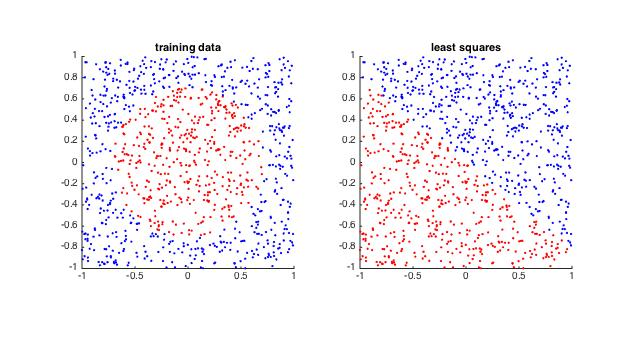
\includegraphics[scale=.8]{hw8_2_truth.jpg}

On the left, the plot is showing the truth. The positive and negative cases were plotted using different colors. From this plot, we know that we need a non-linear decision boundary since there is no straght line solution is going to separate the two classes. \\

\newpage
Here's the plot showing the predicted classification for ridgre regression with Gaussian kernel: 
\begin{center}
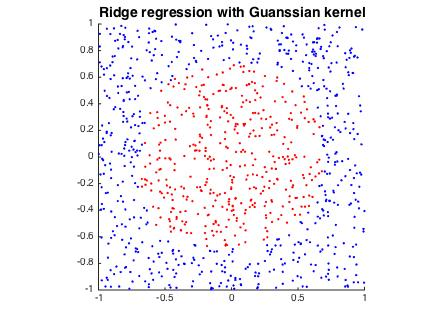
\includegraphics[scale=.8]{hw8_2_GauKerLS.jpg}
\end{center}

The accuracy of ridgre regression with Gaussian kernel is 0.9820, which is much better than the least square solution. 


\newpage
Here's the MATLAB code for Gaussian kernelized ridge
\begin{lstlisting}
clear; close all;clc
training_data
% set lambda
lambda = 1e-5;

%% compute the polynomial kernal
m = size(A,1);
gauKer = nan(m,m);
for i = 1 : m
    for j = 1 : m
        gauKer(i,j) = exp(-.5 * (norm(A(i,:) - A(j,:),2))^2);
    end
end

%% fit the kernelized least square
alpha = inv(gauKer + lambda * eye(size(gauKer))) * b;


%% compute classification accuracy
prediction = nan(m,1);
for i = 1 : m
    temp = 0;
    xnew = A(i,:);
    for j = 1 : m
        temp = temp + alpha(j) * exp(-.5 * (norm(xnew - A(j,:),2) )^2);
    end
    prediction(i) = sign(temp);
end

sum(prediction)
accuracy = sum(prediction == b) / length(b)

%% plot the prediction 
figure; 
hold on;
for i=1:m
    a = A(i,:);
    if prediction(i)==1
        plot(a(1),a(2),'b.');
    else
        plot(a(1),a(2),'r.');
    end
end
axis('square')
title('Ridge regression with Guanssian kernel', 'fontsize',14)
\end{lstlisting}

%----------------------------------------------------------------------------------------
%	PROBLEM 3
%----------------------------------------------------------------------------------------
\newpage
\section*{Question3}
\textbf{Design a classifier using the polynomial kernel}
$$ k(a_i,a_j) = (a_i^Ta_j +1)^2 $$
\textbf{and regularization parameter $\lambda = 10^{-5}$. Compare its classification performance of the training data to the least sqaure and the Gaussian kernel classifier. }\\

Here's the plot showing the predicted classification: 
\begin{center}
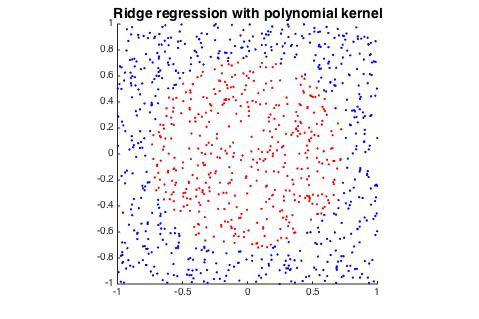
\includegraphics[scale=.8]{hw8_3_polyKerLS.jpg}
\end{center}

The accuracy of ridgre regression with polynomial kernel is 0.9650, which is much better than the least square solution. It is slightly worse than the Gaussian kernel but I am not sure if the statistically difference is significant or not.


\newpage
Here's the MATLAB code for polynomial kernelized ridge 
\begin{lstlisting}
clear; close all;clc
training_data
% set lambda
lambda = 1e-5;

%% compute the polynomial kernal
m = size(A,1);
ker = nan(m,m);
for i=1:m
    for j=1:m
        ker(i,j) = (dot(A(i,:), A(j,:)) +1 )^2;
    end
end

% %% test kernel 
% phi = [A(:,1).^2 sqrt(2).*A(:,1).*A(:,2) A(:,2).^2 sqrt(2)*A(:,1) sqrt(2)*A(:,2) ones(m,1)];
% kert = phi * phi';
% [ker(:,1) kert(:,1)]

%% fit the kernelized least square
alpha = inv(ker + lambda * eye(size(ker))) * b;

%% compute classification accuracy
prediction = nan(m,1);
predict_t = nan(m,1);
% compute the kernel LS prediction 1 by 1
for i = 1 : m
    temp = 0; 
    xnew = A(i,:);
    % compute the kernel LS prediction for 1 example
    for j = 1 : m
        temp = temp + alpha(j) * (dot(xnew, A(j,:)) +1 )^2;
    end
    prediction(i) = sign(temp);
end

accuracy = sum(prediction == b) / length(b)

%% plot the prediction 
figure; 
hold on;
for i = 1 : m
    a = A(i,:);
    if prediction(i) == 1
        plot(a(1),a(2),'b.');
    else
        plot(a(1),a(2),'r.');
    end
end
axis('square')
title('Ridge regression with polynomial kernel', 'fontsize',14)
\end{lstlisting}


%----------------------------------------------------------------------------------------
%	PROBLEM 4
%----------------------------------------------------------------------------------------
\newpage
\section*{Question4}
\textbf{Now experiment with these methods in the following way. Generate different sized sets of training data: m = 10, 100, 1000. Design the three types of classifiers using these data. Test the performance of the classifiers using independent sets of data of size 100. For each training data size, repeat the training and testing 100 times and average the results. This will provide a good indication of how the different approaches perform with different amounts of training data. Summarize your results by reporting the average test error for each of the three methods and each of the three training set sizes.}\\


Here's the plot that shows the comparison of the performance. 
\begin{center}
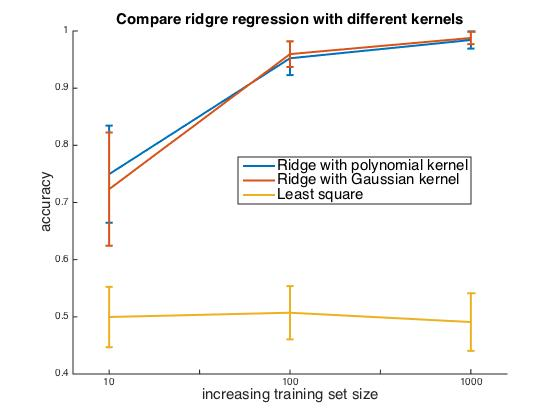
\includegraphics[scale=.5]{hw8_4_compareRidge.jpg}
\end{center}

The Y axis shows the accuracy, and the X axis is showing increasing size of the training set, ranges from 10 to 1000. I am comparing standard least square and ridge regression with polynomial kernel or Gaussian kernel. They were visualized by different colored lines. The error bar is showing one standard deviation. \\

We can see that when there are more training examples, ridge regression with either Gaussian or polynomial kernel performed better. In particular, the performance of both kernelized ridge reached the ceiling in this setting when the training size is 1000. Compare to the polynomial kernel, it seems that Gassian kernel is better when there were 1000 training examples, and it is worse when there were 10 training examples but the statistical difference was insignificant. \\

On the other hand, the performance of standard least square did not increase when there are more training examples. \\

\newpage
Here's the MATLAB code I used for comparing the 3 method on one train-test session. 
\begin{lstlisting}
%% compare 2 kernel methods 
function [accuracy] = compare3methods(trainingSetSize)
% generate training and testing data
[A, b] = genTraining_data(trainingSetSize, 0);
[Atest, btest] = genTraining_data(100, 0);
% set lambda
lambda = 1e-5;
%% compute the polynomial kernal
m = size(A,1);
ker.poly = nan(m,m);
ker.gaus = nan(m,m);
for i=1:m
    for j=1:m
        ker.poly(i,j) = (dot(A(i,:), A(j,:)) +1 )^2;
        ker.gaus(i,j) = exp(-.5 * (norm(A(i,:) - A(j,:),2))^2);
    end
end

%% fit the kernelized least square
alpha.poly = inv(ker.poly + lambda * eye(size(ker.poly))) * b;
alpha.gaus = inv(ker.gaus + lambda * eye(size(ker.gaus))) * b;

%% compute classification accuracy
prediction.poly = nan(size(Atest,1),1);
prediction.gaus = nan(size(Atest,1),1);
% compute the kernel LS prediction 1 by 1
for i = 1 : size(Atest,1)
    xnew = Atest(i,:);
    % compute kernel LS prediction for 1 example (polynomial)
    temp = 0; 
    for j = 1 : m
        temp = temp + alpha.poly(j) * (dot(xnew, A(j,:)) +1 )^2;
    end
    prediction.poly(i) = sign(temp);    
    % compute kernel LS prediction for 1 example (gaussian)
    temp = 0;
    for j = 1 : m
        temp = temp + alpha.gaus(j) * exp(-.5 * (norm(xnew - A(j,:),2) )^2);
    end
    prediction.gaus(i) = sign(temp);    
end

%% fit standard LS
wts.ls = pinv(A)*b;
prediction.ls = sign(Atest * wts.ls);

%% compute accuracy for the 2 methods
accuracy.p = sum(prediction.poly == btest) / length(btest);
accuracy.g = sum(prediction.gaus == btest) / length(btest);
accuracy.ls = sum(prediction.ls == btest) / length(btest);
end

\end{lstlisting}




%----------------------------------------------------------------------------------------
%	PROBLEM 5
%----------------------------------------------------------------------------------------
\newpage
\section*{Question5}
\textbf{Now tackle the problem using hinge loss instead of squared error loss. You do this using the Matlab function svmtrain, another package, or by writing your own code (e.g., GD or SGD). Generate different sized sets of training data: m = 10, 100, 1000. Design SVM classifiers using both Gaussian and polynomial kernels. Test the performance of the classifiers using independent sets of data of size 100. For each training data size, repeat the training and testing 100 times and average the results. Compare your results to those obtained using least squares.}\\


Here's the plot showing the three methods I tried: 
\begin{center}
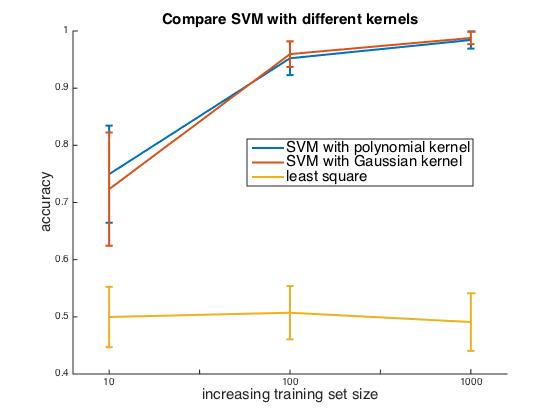
\includegraphics[scale=.5]{hw8_5_compareSVM.jpg}
\end{center}

The Y axis shows the accuracy, and the X axis is showing increasing size of the training set, ranges from 10 to 1000. I am comparing the least square solution with support vector machine with polynomial kernel and Gaussian kernel. They were visualized by different colored lines. The error bar is showing one standard deviation. \\

The story is pretty similar with the what we saw in question 4. SVM with both kernels performed better when there are more training examples. The performance of both kernelized SVM reached the ceiling when the training size is 1000. On the other hand, the performance of standard least square did not increase when there are more training examples. Indeed, standard least square always give us chance performance. \\

\newpage

Here's the MATLAB code for comparing the 3 methods, used in question 5. I used matlab svmtrain package. 
\begin{lstlisting}
function accuracy = compare3kernels_svm(m)
% generate training and test data
% m = 100;
m_test = 100;
[A,b] = genTraining_data(m,false);
[Atest,btest] = genTraining_data(m_test,false);

%% compute svm with rbf or poly kernel
% subplot(1,2,1)
svm.rbf = svmtrain(A,b, 'ShowPlot', 0, 'kernel_function', 'rbf');
% subplot(1,2,2)
svm.poly = svmtrain(A,b, 'ShowPlot', 0, 'kernel_function', 'polynomial');

%% compute the accuracy for rbf and poly kernelized svm
prediction.rbf = nan(m_test,1);
prediction.poly = nan(m_test,1);
for i = 1 : m_test
    Xnew = Atest(i,:);
    prediction.rbf(i) = svmclassify(svm.rbf,Xnew,'ShowPlot',0);
    prediction.poly(i) = svmclassify(svm.poly,Xnew,'ShowPlot',0);
end
% compute accuracy
accuracy.rbf = sum(prediction.rbf == btest) / length(btest);
accuracy.poly = sum(prediction.poly == btest) / length(btest);

%% fit standard least square model and compute the accuracy
wts.ls = pinv(A) * b;
prediction.ls = sign(Atest*wts.ls);
accuracy.ls = sum(prediction.ls == btest)/length(btest);
end
\end{lstlisting}


%----------------------------------------------------------------------------------------
%	PROBLEM 6
%----------------------------------------------------------------------------------------
\newpage
\section*{Question6}
\textbf{Consider the problem of trying to predict whether a person is a basketball player based on height. The training data consists of four people with heights of 5'10", 5'11', 6'1" and 6'10", and the latter two are basketball players. What classification rule do you obtain by minimizing hinge loss instead of squared error loss?}\\

First of all, let me convert feet to meters, and define the resulting matrix as my data matrix\\
$$
\begin{bmatrix}
5'10"	\\
5'11'	\\
6'1" 	\\
6'10"
\end{bmatrix}
\rightarrow
\begin{bmatrix}
1.78		\\
1.8		\\
1.85	 	\\
2.08
\end{bmatrix}
=: X
$$

And define y as the following: 

$$
\begin{bmatrix}
\text{not a basketball player}	\\
\text{not a basketball player}	\\
\text{basketball player} 	\\
\text{basketball player}
\end{bmatrix}
\rightarrow
\begin{bmatrix}
-1		\\
-1		\\
1	 	\\
1
\end{bmatrix}
=: y
$$
Then we can use X and y to do classification. Now I want to compare LS boundary with the SVM boundary. \\

In the following plot, the LS and SVM boundaries were plotted with 'x' in different colors and data were shown using circles with different colors. 

\begin{center}
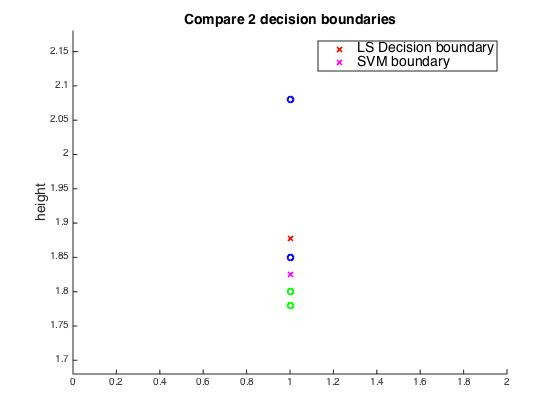
\includegraphics[scale=.5]{hw8_6_2boundaries.jpg}
\end{center}

Because LS has positive cost for examples that are classified too well, the very tall guy is pulling the decision boundary up, resulting a bad boundary. The SVM boundry has zero cost for correctly classified examples so the decision boundary is insensitive to the very tall guy. 

\newpage

Here's the matlab code that generate the simulation in question 6. 

\begin{lstlisting}
clear all;close all;clc;
X = [1 1 1 1; 1.78 1.8 1.85 2.08]';
y = [-1 -1 1 1]';

%% fitting LS
w.ls = inv(X' * X) * X' * y;
sign(X * w.ls)

%% fit svm
tau = 0.03;
lambda  = 0;
w.svm = zeros(size(X,2),1);
numIters = 100000;
% implement gradient decent
for i = 1 : numIters
    change = zeros(size(X,2),1);
    % accumulate the gradient for all training examples
    for j = 1 : length(y)
        if 1 - y(j) * X(j,:) * w.svm > 0 
            change(:) = change(:) - y(j) * X(j,:)';
        end
    end
    % gradient decent update
    w.svm = w.svm - tau * change;
    % 
    fprintf('%d %f \n', i, norm(y - X * w.svm));    
end

%% plot the decision boundary 
hold on
plot(-w.ls(1)/w.ls(2), 'rx', 'linewidth', 2)
plot(-w.svm(1)/w.svm(2), 'mx', 'linewidth', 2)

title('Compare 2 decision boundaries' ,'fontsize', 14)
ylabel('height', 'fontsize', 14)
legend({'LS Decision boundary', 'SVM boundary'} ,'fontsize', 14)
ylim([min(X(:,2))-.1 max(X(:,2))+.1])
% plot the points 
for i = 1 : size(X,1)
    if y(i) >0
        plot(X(i,2), 'bo', 'linewidth', 2)
    else
        plot(X(i,2), 'go', 'linewidth', 2)
    end
end
hold off
\end{lstlisting}

%----------------------------------------------------------------------------------------
%	PROBLEM 7
%----------------------------------------------------------------------------------------
\newpage
\section*{Question7}
\textbf{If you consider the dual solution in this case, which values of $\alpha \in \mathbb{R}^4$ are nonzero (i.e. what are the support vectors? )}\\

The alpha associated with the 2nd and the 3rd examples will be non-zero. Namely, the example that is closest from the svm decision boundary on each side are the support vectors. 




%----------------------------------------------------------------------------------------
%	PROBLEM 8
%----------------------------------------------------------------------------------------
\newpage
\section*{Question8}
\textbf{ The standard hinge loss is linearly decreasing up to 1 and then exactly 0 after. Let $t_0$ denote the point where the hinge loss first becomes 0. Does the solution change if you shift the $t_0$ within the range $t_0 \in [0, 1]$?}\\

Yes it would change. \\

When $t_0$ is 1, things larger than 1 has 0 loss, things less 0 than has a high cost, and things with in [0,1] has a small loss. Therefore, we are acutally penalizing things that are classified correctly with in [0,1]. This is really saying that we want more than merely classifying things correctly, we want to be right by at least 1, which creates the margin. \\


If $t_0$ shrinks, then the margin would shrink. Consider the extreme when $t_0$ is 0, then everything classified corrected would have no cost. Assume the data are linearly separable, there can exist many decision boundaries with zero loss, and the classifier no longer care about maximizing the margin. 




\end{document}